\documentclass[11pt]{article}
\usepackage{deauthor,times,graphicx,subcaption}
%\graphicspath{{figs/}}


\begin{document}
\title{Operating systems support for data management \\ on modern hardware}
\author{Jana Giceva \\ Imperial College London \\ j.giceva@imperial.ac.uk}
\maketitle

\begin{abstract}
For decades, database management systems have found the generic interface, policies and mechanisms offered by 
conventional operating systems at odds with the need for efficient utilization of hardware resources. The 
existing approach from the OS-side of "one-size-fits-all" interface and policies fails to meet modern data 
management workload's performance expectations, and the "overwriting the OS policies" approach from the 
DB-side does not scale with the increasing complexity of modern hardware and deployment trends.
 
In this article, we present two approaches on how to improve the systems support for database engines. First, 
we extend the OS with a policy engine and a declarative interface to improve the knowledge transfer between 
the two systems. Such extensions allow for easier deployment on different machines, more robust execution 
in noisy environments and better resource allocation without sacrificing performance guarantees. Second, 
we show how we leverage a novel OS architecture to develop customized OS kernels that meet the needs of 
data management workloads. Finally, we discuss how both approaches can help to address the pressing 
challenges for data processing on heterogeneous hardware platforms.
\end{abstract}

%\section{Introduction}
\label{seC:intro}
% Interpretability and nutritional labels, generally

An essential ingredient of successful machine-assisted decision-making, particularly in high-stakes decisions, is interpretability --– allowing humans to understand, trust and, if necessary, contest, the computational process and its outcomes.   These decision-making processes are typically complex:  carried out in multiple steps, employing models with many hidden assumptions, and relying on datasets that are often repurposed --- used outside of the original context for which they were intended.\footnote{See Section 1.4 of Salganik's ``Bit by Bit''~\cite{salganik} for a discussion of data repurposing in the Digital Age, which he aptly describes as "mixing readymades with custommades.''}  In response, humans need to be able to determine the ``fitness for use'' of a given model or dataset, and to assess the methodology that was used to produce it.  

To address this need, we propose to develop interpretability and transparency tools based on the concept of a {\em nutritional label}, drawing an analogy to the food industry, where simple, standard labels convey information about the ingredients and production processes. Short of setting up a chemistry lab, the consumer would otherwise have no access to this information. Similarly, consumers of data products cannot be expected to reproduce the computational procedures just to understand fitness for their use.   Nutritional labels, in contrast, are designed to support specific decisions by the consumer rather than completeness of information.  A number of proposals for hand-designed nutritional labels for data, methods, or both have been suggested in the literature\cite{DBLP:journals/corr/abs-1803-09010,DBLP:journals/corr/abs-1805-03677,DBLP:conf/fat/MitchellWZBVHSR19}; we advocate deriving such labels automatically or semi-automatically as a side effect of the computational process itself, embodying the paradigm of {\em interpretability-by-design}. 

Interpretability means different things to different stakeholders, including individuals being affected by decisions, individuals making decisions with the help of machines, policy makers, regulators, auditors, vendors, data scientists who develop and deploy the systems, and members of the general public.  Designers of nutritional labels must therefore consider {\em what} they are explaining,  {\em to whom}, and {\em for what purpose}.  In the remainder of this section, we will briefly describe two regulatory frameworks that mandate interpretability of data collection and processing to members of the general public, auditors, and regulators,  where nutritional labels offer a compelling solution (Section~\ref{sec:intro:reg}).  We then discuss interpretability requirements in data sharing, particularly when data is altered to protect privacy or mitigate bias (Section~\ref{sec:intro:synth}).

\subsection{Regulatory Requirements for Interpretability}
\label{sec:intro:reg}

The European Union recently enacted a sweeping regulatory framework known as the General Data Protection Regulation, or the GDPR~\cite{gdpr}.  The regulation was adopted in April 2016, and became enforceable about two years later, on May 25, 2018.  The GDPR aims to protect the rights and freedoms of natural persons with regard to how their personal data is processed, moved, and exchanged (Article 1).  The GDPR is broad in scope, and applies to ``the processing of personal data wholly or partly by automated means'' (Article 2), both in the private sector and in the public sector.  Personal data is broadly construed, and refers to any information relating to an identified or identifiable natural person, called the {\em data subject} (Article 4).  

According to Article 4, lawful processing of data is predicated on the data subject's {\em informed consent}, stating whether their personal data can be used, and for what purpose (Articles 6, 7).
Further,  data subjects have {\em the right to be informed} about the collection and use of their data.~\footnote{\url{https://gdpr-info.eu/issues/right-to-be-informed/}}
Providing insight to data subjects about the collection and use of their data requires technical methods  that support interpretability.  

Regulatory frameworks that mandate interpretability are also starting to emerge in the US.  New York City was the first US municipality to pass a law (Local Law 49 of 2018)~\cite{Vacca}, requiring that a task force be put in place to survey the current use of ``automated decision systems'' (ADS) in city agencies. ADS are defined as ``computerized implementations of algorithms, including those derived from machine learning or other data processing or artificial intelligence techniques, which are used to make or assist in making decisions.''   The task force is developing recommendations for enacting algorithmic transparency by the agencies, and will propose procedures for: (i) requesting and receiving an explanation of an algorithmic decision affecting an individual (Section 3 (b) of Local Law 49); (ii) interrogating ADS for bias and discrimination against members of legally protected groups, and addressing instances in which a person is harmed based on membership in such groups (Sections 3 (c) and (d)); (iii) and assessing how ADS function and are used, and archiving the systems together with the data they use (Sections 3 (e) and (f)).

Other government entities in the US are following suit.  Vermont is convening an Artificial Intelligence Task Force to ``... make recommendations on the responsible growth of Vermont’s emerging technology markets, the use of artificial intelligence in State government, and State regulation of the artificial intelligence field.''~\cite{Vermont}.  Idaho’s legislature has passed a law that eliminates trade secret protections for algorithmic systems used in criminal justice~\cite{Idaho}.  In early April 2019, Senators Booker and Wyden introduced the Algorithmic Accountability Act of 2019 to the US Congress~\cite{BookerWydenClarke}. The Act, if passed, would use ``automated decision systems impact assessment'' to address and remedy harms caused by algorithmic systems to federally protected classes of people. The act empowers the Federal Trade Commission to issue regulations requiring larger companies to conduct impact assessments of their algorithmic systems.

The use of nutritional labels in response to these and similar regulatory requirements can benefit a variety of stakeholders.  The designer of a data-driven algorithmic method may use them to validate assumptions, check legal compliance, and tune parameters.  Government agencies may exchange labels to coordinate service delivery, for example when working to address the opioid epidemic, where  at least three sectors must coordinate: health care, criminal justice, and emergency housing, implying a global optimization problem to assign resources to patients effectively, fairly and transparently. The general public may review labels to hold agencies accountable to their commitment to equitable resource distribution. 


\subsection{Interpretability with Semi-synthetic Data}
\label{sec:intro:synth}

%Datasets are now increasingly used to train models to make decisions once made by humans.  In these automated systems, biases in the data are propagated and amplified with no human in the loop.  The bias, and the effect of the bias on the quality of decisions made, is not easily detectable due to the relative opacity of the system.  

A central issue in machine-assisted decision-making is its reliance on historical data, which often embeds results of historical discrimination, also known as {\em structural bias}.   As we have seen time and time again, models trained on data will appear to work well, but will silently and dangerously reinforce discrimination~\cite{propublicaJ,amazon_hiring,amazon_delivery}.  Worse yet, these models will legitimize the bias --- ``the computer said so.''  Nutritional labels for data and models are designed specifically to mitigate the harms implied by these scenarios, in contrast to the more general concept of ``data about data.''

Good datasets drive research: they inform new methods, focus attention on important problems, promote a culture of reproducibility, and facilitate communication across discipline boundaries.  But research-ready datasets are scarce due to the high potential for misuse. Researchers, analysts, and practitioners therefore too often find themselves compelled to use the data they have on hand rather than the data they would (or should) like to use.  For example, aggregate usage patterns of ride hailing services may overestimate demand in early-adopter (\ie wealthy) neighborhoods, creating a feedback loop that reduces service in poorer neighborhoods, which in turn reduces usage.  In this example, and in many others, there is a need to alter the input dataset to achieve specific properties in the output, while preserving all other relevant properties.  We refer to such altered datasets as \textit{semi-synthetic}.

Recent examples of methods that produce semi-synthetic data include database repair for causal fairness~\cite{DBLP:conf/sigmod/SalimiRHS19}, database augmentation for coverage enhancement~\cite{DBLP:conf/icde/AsudehJJ19}, and privacy-preserving and bias-correcting data release~\cite{DBLP:conf/ssdbm/PingSH17,DBLP:conf/vldb/RodriguezSPSH18}. A semi-synthetic datasets may be altered in different ways.  Noise may be added to it to protect privacy, or statistical bias may be removed or deliberately introduced.  When a dataset of this kind is released, its composition and the process by which it was derived must be made interpretable to a data scientist, helping determine fitness for use.  For example, datasets repaired for racial bias are unsuitable for studying discrimination mitigation methods, while datasets with bias deliberately introduced are less appropriate for research unrelated to fairness.   This gives another compelling use case for nutritional labels.

%To make our discussion more concrete, let us consider data scientists who must identify datasets appropriate for their task.  This is particularly important when semi-synthetic datasets are being released, to which noise is added to protect privacy, or statistical bias is removed or deliberately introduced.  For example, datasets repaired for racial bias are unsuitable for studying discrimination mitigation methods, while datasets with bias deliberately introduced are less appropriate for research unrelated to fairness.  




\section{Introduction}

Generally, today's operating systems multiplex applications with little to no information 
about their requirements. They migrate, preempt, and interrupt threads on various cores,
trying to optimize some system-wide objectives (e.g., load balancing the work queues
on individual cores and across the NUMA nodes~\cite{Lozi:eurosys16}). As such, the OS
has no notion about how its decisions affect the performance of the applications 
primarily due to the limited communication between the two layers~\cite{cod:2013}. 

As a result, database engines that run on commodity operating systems often experience
performance problems, which are caused by the generic OS policies~\cite{Stonebraker:1981}. 
First, when executing in a noisy environment alongside other applications, the 
default OS policies for resource management can often cause performance 
degradation~\cite{Shoal} or inefficiencies in resource usage~\cite{Giceva:damon16,Lozi:eurosys16}. 
Second, even when running in isolation, databases often override the generic OS policies
(e.g., by pinning threads to cores, allocating memory from a particular NUMA node, or 
pinning pages to avoid swapping, etc.~\cite{Porobic:icde14,Kimura:2015}). The 
problem with such user-side optimizations is that they are often tailored to a 
specific architecture, which makes portability to other platforms a daunting
task~\cite{Makreshanski:vldb15,satish:sigmod10}. 
Third, frequently the applied optimizations are fragile as they rely on assumptions on
what the OS kernel mechanisms and policies do (e.g., HyPer~\cite{HyPer} leverages
an efficient OS-assisted snapshotting). Consequently, any change in the OS policies
can cause performance bugs that are difficult to identify and debug.

In light of modern hardware trends of increased hardware heterogeneity and machine 
diversity, pushing all the complexity up to the developer or within the database 
engine does not scale. Furthermore, as databases are often deployed in the cloud,
alongside other applications and tasks, they can no longer assume to have full
ownership of the underlying machine's resources and any scheduling decision they do
may be at odds with the noisy system environment and result in unpredictable 
performance.

In this article we argue that it is time to revisit the interface between operating
systems and databases and address the modern challenges in a holistic manner crossing
various layers across the systems stack. More specifically, we propose a solution that
first addresses the semantic gap that exists between the database engine and the 
operating system by leveraging (1) a powerful declarative interface between the two
layers allowing for bi-directional information flow, and (2) an OS policy engine that 
unifies the knowledge present in the database (workload characteristics, access patterns,
cost models, data distribution, etc.) with the knowledge of the OS about the 
underlying hardware and the runtime system-state. 
Furthermore, we present a novel OS architecture that allows for OS kernel customization
(i.e., policies, mechanisms and services) based on the specific requirements of 
the database system or its workloads. Our design is inspired by recent advancements
in operating systems, which enable systems to run a specialized kernel on a subset
of the resources on a given machine. This enables the database to get considerably
more control over the full OS stack, which can then be tuned to achieve both better
performance and stronger guarantees. 
Finally, we argue how both design principles are suitable to target modern hardware 
resource dis-aggregation challenges, raising a few interesting research directions.

%
\section{Background on Privacy-Sensitive Mobile Contact Tracing}

The key building block for Privacy-Sensitive Mobile Contact Tracing (PS-MCT) is a subtle combination of radio protocols, cryptography, and risk-calculation.  
Phones have a short-range radio, Bluetooth, used to connect to nearby devices.  
To make those connections it periodically broadcasts tiny bits of information. 
The PS-MCT protocols leverages this short-range background broadcast to resolve nearby individuals.\shankari{Is this the final term we decided on? I recall some pushback from David on the term, and I don't remember this as one of the options. Since our current focus is on the idea and not on a working system, it seems like it is a good idea to get the terminology right}


In the Apple-Google Exposure Notification (AGEN) protocol, each phone generates a daily secret key called a Temporary Exposure Key (TEK).
Then every 15 minutes the phone uses the TEK to generate a new 16 byte Rolling Proximity Identifier (RPI). The RPI sequence is generated using a cryptographic hash function, so it does not carry any information about the source individual.  
The current RPI is then continuously broadcast every few hundred milliseconds.
All phones log the RPIs they hear for future exposure analysis.  
Because the RPI is continuously changing, it also cannot be easily tracked.


When someone tests positive they can \textbf{anonymously} publish the daily keys (TEKs) from the days when they were contagious.  
The confirmed positive collection of TEKs is called a Diagnosis Key in the AGEN protocol.  
The Diagnois Keys are published by sharing them with a trusted server which publishes the TEKs for download.
Others can obtain these keys and use the same cryptographic hash functions to recreate the sequence of RPIs. This sequence, combined with some region-specific weights, can determine if they encountered any infected individuals.  
This entire process is accomplished within the Android and iOS operating systems. Government sanctioned apps are only responsible for authenticating infected individuals and, with user permission, publishing the keys. 

It is important to note the distinction between policy and mechanism. The AGEN protocol (and the extensions proposed in this paper) provide a mechanism to detect and notify users about exposure risk, but it is up to public health authorities to define what constitutes an exposure. This distinction is explored in more detail in section \ref{sec:commons}.




\section{Background}

Databases and operating systems have a decades-long conflict when it comes to resource management and 
scheduling. Even though they initially started with the same goal -- providing efficient access 
of data written in files -- they took different approaches to addressing the problem. For many 
years this was not perceived as an issue as the two systems were targeting different 
workloads and machines. This shaped the role of monolithic databases and operating systems
as we know them today. 
However, the economic advantage of off-the-shelf hardware has led to today's situation where a 
database runs on top of conventional OS. The key problem is that the OS works with very little 
knowledge about the workload requirements and properties. Its primary role is to schedule 
resources among multiple applications and to provide isolation protection. As such, it sees the 
database as yet another program and offers the same generic mechanisms and policies, which often
lead to sub-optimal performance numbers.

Recent trends in both hardware architectures and resource dis-aggregation over fast network 
interconnects as well as economies of scale and deployment in the cloud are pressing both 
layers of the system stack to rethink their internal designs. The last decade, in particular, 
has seen profound changes in the available hardware as we reached the power wall limitation
and CPU frequencies stopped scaling. In response, hardware architects introduced multiple 
cores, heterogeneous compute resources and accelerators. Similarly, with the rise of the 
memory wall and the gap between DRAM and CPU frequencies, machines emerged with more 
complex cache hierarchies, non-uniform cache coherent memory, etc. Consequently, the 
system software (both DBs and OSs) has to adapt and embrace the new hardware landscape 
as an opportunity to rethink its architecture model and design principles.
For example, to improve performance, novel scheduling decisions within a database
engine~\cite{Leis:sigmod14,Porobic:icde14} and certain relational algorithms has 
shifted towards hardware awareness in modern machines~\cite{Polychroniou:2014,balkesen:15,wassenberg2011,muller:16}. 
Optimal use of resources today requires detailed knowledge of the underlying hardware 
(e.g., memory affinities, cache hierarchies, interconnect distances). 
Absorbing such complexity has now become the burden of the programmer and the 
problem gets further aggravated with the increasing diversity of micro-architectures. 

On the deployment side, in the age of cloud and server consolidation, databases can 
no longer assume to have a complete physical machine to themselves. They are 
increasingly more often deployed and offered as services on the cloud, where they
run alongside other applications. Consequently, the carefully constructed internal 
model of machine resources a database typically uses to plan the execution of its 
query plans and physical relational operators has become highly dependent on the 
runtime state of the whole machine. This state, however, is unknown to the database
and is only available in the operating system which has an overview of all 
active applications and orchestrates the resource allocation. 

In that context, we make the following observations. First, databases can no longer 
take full ownership of resource management, allocation and scheduling, partly because 
of increasing hardware complexity and portability issues, and partly because databases
today are running in noisy environments (e.g., in the cloud), alongside other applications.
Second, there is a big semantic gap between what each layer of the system stack knows --
the database engine about its workload properties and requirements and the operating 
systems about the underlying hardware and runtime system-state -- and the rigid 
interface between them does not allow for rich information flow. Fourth, the 
one-size-fit-all generic policies and mechanisms offered by the OS for a wide range 
of workloads do not work for performance sensitive applications, like data processing 
engines. And fifth, the heavy OS stack is no longer suitable for the new generation 
hardware, with heterogeneous (rack-scale) resource dis-aggregation. These are the 
issues we address as part of our work and discuss in the article.

%%!TEX root=../2022_IEEE_DEB_Vizier.tex

% %%%%%%%%%%%%%%%%%%%%%%%%%%%%%%%%%%%%%%%%
% \begin{figure}[t]
%   \centering
%   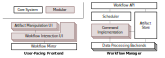
\includegraphics[width=0.7\textwidth]{graphics/systemarch}\\[-5mm]
%   \caption{Vizier's architecture, comprised of a user-facing frontend component and a backend component.}\label{fig:vizier-architecture}
% \end{figure}
% %%%%%%%%%%%%%%%%%%%%%%%%%%%%%%%%%%%%%%%%

%%%%%%%%%%%%%%%%%%%%%%%%%%%%%%%%%%%%%%%%%%%%%%%%%%%%%%%%%%%%%%%%%%%%%%%%%%%%%%%%
\pagebreak[4]
\subsection{Solution Overview}
\label{sec:solution-overview}

%%%%%%%%%%%%%%%%%%%%%%%%%%%%%%%%%%%%%%%%
\begin{wrapfigure}[12]{r}[0pt]{12cm}
  \centering
  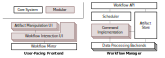
\includegraphics[width=0.7\textwidth]{graphics/systemarch}\\[-5mm]
  \caption{Vizier's architecture, comprised of a user-facing frontend component and a backend component.}\label{fig:vizier-architecture}
\end{wrapfigure}
%%%%%%%%%%%%%%%%%%%%%%%%%%%%%%%%%%%%%%%%
An overview of Vizier's architecture is shown in \Cref{fig:vizier-architecture}.
Addressing requirement \textbf{W1}, the central abstraction in Vizier is a workflow: a linear sequence of steps. % taken by the user in pursuit of a specific objective.
Unlike classical workflow systems, Vizier does not require users to explicitly declare information flow between steps.
Rather Vizier borrows the model employed in popular computational notebooks like Jupyter, where inter-cell communication occurs through a global state (artifacts) passed sequentially through steps.
Following notebook conventions, we refer to these steps as \emph{cells}, and the global state as a \emph{scope}, a map from artifact name to the version of the artifact valid at this point in the workflow. Vizier stores artifacts in common formats through a versioned \textbf{Artifact Store} (\Cref{sec:data-artifacts}), addressing requirement \textbf{A2}.
In \Cref{sec:vizier-workflows}, we formalize Vizier's workflow model, and show how we satisfy requirement \textbf{W3} by instrumenting how each cell interacts with the scope, allowing us to determine what artifact versions are valid.

Vizier's workflow semantics, paired with the versioned artifact store and workflow versioning (\Cref{sec:vizier-history}) addresses requirement \textbf{W2}. % as notebooks have a natural concept of logical order (the order of cells in the notebook) that can be adjusted over time.
% Adding workflow versioning  is sufficient to fully address the requirement.
In contrast, classical notebooks like Jupyter or Zeppelin rely on the global state of an interpreter for inter-cell communication.
Reverting this state to an earlier revision is challenging~\cite{zelnicki:2017:nodebook}, limiting their ability to satisfy requirement \textbf{W3}.
Vizier instead relies on its versioning system, allowing its \textbf{Scheduler} to automatically detect and re-evaluate stale cells (\Cref{sec:vizier-scheduler}).
To address requirement \textbf{A3}, we designed a light-weight uncertain data model that is implemented in Vizier in the form of \textit{caveats}, annotations on data that indicate uncertain values and rows  (\Cref{sec:data-docum-error}).

Addressing requirement \textbf{A1} requires modularity in both Vizier's front- and back-end components.
First, the user's interactions with a workflow and artifacts, whether through a scripting language, graphical interaction, or any other modality, need to be captured for replay (simultaneously addressing requirement \textbf{A4}). In Vizier this is achieved by requiring that every update to an artifact made through a particular modality has to be reflected as an operation in the workflow, i.e., a data update is translated into a workflow update.
Vizier manages a collection of \textbf{Command Implementations} that implement the logic behind these artifact transformations (\Cref{sec:multimodality}).
To streamline the implementation of commands, Vizier's data formats and transformations are built over standard \textbf{Data Processing Backends} like Apache Spark.
% For example, Vizier supports fine-grained provenance over datasets by encoding them as Spark data frames.

The frontend is implemented over a \textbf{Workflow Mirror} that uses websockets to reflect a live view of the workflow the user is editing.
Vizier automatically derives a default \textbf{Artifact Manipulation User Interface} for its notebook interface from each command's parameter schemas. This interface suffices for many templated commands, but the frontend can be further extended to provide a more customized experience, for example for Spreadsheet-style direct manipulation of data (\Cref{sec:spreadsheets}).
As illustrated in \Cref{fig:screenshot}, the frontend displays three \textbf{Workflow Interaction User Interfaces} by default: (i) A direct display of the workflow as a notebook, (ii) a table of contents summary of the notebook, including highlighting from documentation, and (iii) a list of artifacts derived by the notebook.
Several of these components, including the notebook and the artifact list provide access to direct manipulation interfaces.
Additional views currently implemented in Vizier include: (iv) A caveat view (\Cref{sec:data-docum-error}) that shows and tracks potential errors in the workflow and data, (v) a history view that shows the evolution of the workflow over time, and (vi) a data provenance subway diagram view.

%%%%%%%%%%%%%%%%%%%%%%%%%%%%%%%%%%%%%%%%%%%%%%%%%%%%%%%%%%%%%%%%%%%%%%%%%%%%%%%%
\begin{figure}
  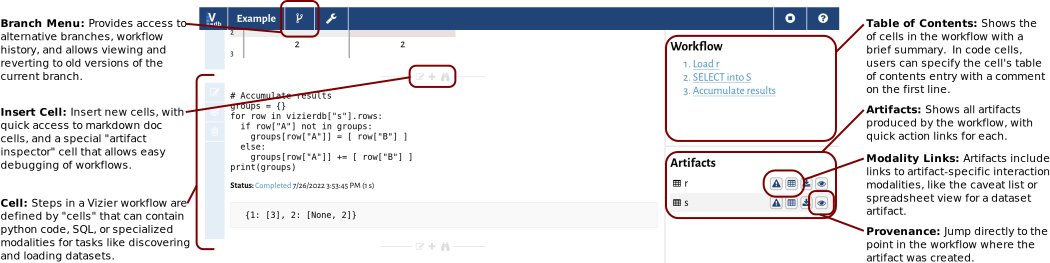
\includegraphics[width=\textwidth]{graphics/screenshot.pdf} 
  \caption{The Vizier User Interface}
  \label{fig:screenshot}
\end{figure}
%%%%%%%%%%%%%%%%%%%%%%%%%%%%%%%%%%%%%%%%%%%%%%%%%%%%%%%%%%%%%%%%%%%%%%%%%%%%%%%%

%%% Local Variables:
%%% mode: latex
%%% TeX-master: "../2022_IEEE_DEB_Vizier"
%%% End:


\section{Overview of proposed solution}

%In our work, we have built a proof-of-concept system that enhances the internal 
%reasoning in the operating system and its computation of resource allocation 
%policies by taking into account the workload properties, as well as enabling 
%for a richer information flow with the database layer. We also revisited the generic 
%OS services and mechanisms and adapted them to better suit the requirements of 
%modern data processing workloads, integrating them as part of a novel OS architecture.

More specifically, we propose customizing the operating system for data-processing applications
and enriching the interface between the two layers to allow for better information flow.
This way the operating system can adjust its allocation policies while reasoning about 
the workload requirements in addition to its optimization for system-wide objectives.
To achieve that, we built a proof-of-concept system that makes the following contributions:

First, we show how the semantic gap between data processing engines and the 
operating system can be avoided by introducing a declarative interface for mutual information
exchange. To do that we explored how to best integrate some of the extensive knowledge 
that a database engine has about its workload requirements (e.g., cost models, data 
dependency graphs, resource requirements, etc.) into the OS. The goal is to enable 
the OS to reason both about the particular requirements and properties of the database 
and about the system-wide and runtime view of the hardware platform and the current
application mix. We achieve that by introducing a policy engine in the OS and a 
resource monitor that facilitates the communication between the two layers. 
A rich \textit{query-based interface} 
then enables any application (including the database) to interact with the policy 
engine. More specifically, it allows the database to (i) query for details about the 
underlying hardware resources, (ii) rely on the policy engine to absorb the hardware 
complexity and diversity, and provide suitable deployment decisions, and (iii) 
push database-specific logic down to the OS in the form of stored procedures that 
enables it to adjust and react to noisy system environments (\S~\ref{sec:policy}). 
The system architecture is shown in Figure~\ref{fig:policy_engine}. 


Second, inspired by the multikernel OS design~\cite{baumann:sosp09}, in \S~\ref{sec:basslet}
we propose a novel OS architecture that enables dynamic partitioning of the 
machine's resources (e.g., CPUs, memory controllers, accelerators, etc.) into a 
\textit{control plane}, running a full-weight operating system along with an OS 
policy engine, and a \textit{compute plane}, consisting of specialized light-weight 
OS stacks. The objective is to enable customization of the compute-plane OS both 
for the properties of the underlying hardware (i.e., potentially heterogeneous
compute units) and for the specific requirements of the workload (e.g., customized 
scheduler or memory management). By design the allocation of resources between the 
control and compute plane is dynamic and can be adapted at runtime based on the 
changing workload requirements. 
To demonstrate the benefits of such control-compute plane OS architecture, we present 
a light-weight OS with a kernel-integrated runtime (Basslet), which we run on the 
compute plane, that is customized for parallel data analytics. 

% \input{policy}

\section{OS policy engine}
\label{sec:policy}

The OS policy engine is designed to enable both the OS itself and the database running on top
to better grasp the properties of the available hardware resources and reason about the 
real-time system state. 

\begin{figure}
  \centering
  \includegraphics[scale=0.6, trim=2cm 8cm 8cm 2cm, clip=true]
    {figs/intro_policyengine}
  \caption{Policy Engine}
  \label{fig:policy_engine}
\end{figure}

More specifically, it consists of a \textit{knowledge base} that contains
information about (1) machine specific facts (e.g., topology of the machine, number of cores and
memory per NUMA node, the cache hierarchy, etc.), (2) application-related facts
(e.g., information whether an application is compute- or memory-bound, sensitive to sharing 
the caches, etc.), and (3) current system-state (e.g., number of active applications, 
their memory usage, etc.). This information is used both by the knowledge base to build
a detailed model of the machine and its resources, and by a set of algorithms and solvers
that compute resource allocation schedules. 
For the knowledge base we borrow and extend the concept of System Knowledge Base (SKB) 
from the Barrelfish OS~\cite{Schuepbach12, barrelfish}, which stores data in the format of
free-form predicates in a Constraint Logic Programming (CLP) engine. This enables various 
solvers to reason about the information available by issuing logical queries to perform 
constraint solving and optimization.

The \textit{resource manager} is responsible for communicating with the applications (in our 
case the database engine), triggering resource allocation computations in the knowledge base,
and executing the decided policies by invoking the available OS mechanisms. 
Often, the policy engine relies on a \textit{resource profiler} to measure the capacities 
of hardware resources (e.g., the maximum attainable DRAM bandwidth achievable per NUMA node), 
monitor their current utilization, and enable applications to measure their resource 
requirements or footprints.

Finally, the new {\it interface} is declarative and allows for richer two-way information exchange 
between the DBMS and the OS policy engine. It covers a wide range of actions from retrieving 
information about the underlying architecture to pushing down application-specific cost-models
and dataflow dependencies so that the OS policy engine can reason about them. Furthermore,
by allowing stored procedures it enables database-specific logic to be computed in 
the OS-side that leverages the most up-to-date system-state. Finally, it supports the 
retrieval of application-specific resource usage profiles as measured by the resource 
profiler and enables a continuous information flow between the two layers at runtime
in the form of notifications and updates. This way the OS can do a better job when 
deploying the application's threads onto a range of different machines and provide 
efficient resource allocation without affecting the application's performance of 
predictability; and the database can adapt itself based on the current system state,
which is especially important in noisy environments. 

%\subsection*{Implementation details}
%For the {\it knowledge base} we borrow and extend the concept of System Knowledge Base (SKB) 
%from the Barrelfish OS~\cite{Schuepbach12, barrelfish}. The SKB stores data in the format of
%free-form predicates in the Constraint Logic Programming (CLP) engine. This enables various 
%solvers to reason about the information available by issuing logical queries to perform 
%constraint solving and optimization. We augmented the knowledge stored in the SKB so that 
%it can be classified into two categories: 
%\begin{enumerate}
%\item {\it system-level facts} -- information about the underlying hardware platform (via resource 
%discovery at runtime and online micro-benchmarks) and the system state (via book-keeping of the
%running tasks and their resource usage/assignment), and 
%\item {\it application-specific facts} -- information about the application itself. 
%For instance, either application's properties that an OS can easily understand 
%(e.g., CPU-bound, maximum degree of parallelism, etc.) or that are specific to 
%the application's domain (e.g., dataset size, latency SLOs, etc.). The latter type 
%can only be leveraged by application-specific \textit{stored procedures} that 
%compute system-level properties (e.g., minimum number of cores).
%\end{enumerate}
%As such the SKB is the reactive component of the policy engine that can be seen as a 
%repository and a calculation engine for system knowledge. It is complemented by the
%{\it resource manager}, which is the active component that triggers re-computation of the 
%resource allocation as soon as a new task enters and registers in the system. It is also 
%responsible for implementing the resulting OS policy using the available OS mechanisms. 
%
%The {\it interface} between the database engine and the OS policy engine provides support 
%for knowledge exchange that covers a range of actions from retrieving information about 
%the underlying architecture to pushing down application-specific cost-models and 
%dataflow dependencies so that the OS policy engine can reason about them. Furthermore,
%by allowing stored procedures it enables database-specific logic to be computed in 
%the OS-side that leverages the most up-to-date system-state. Finally, it supports the 
%retrieval of application-specific resource usage profiles as measured by the resource 
%profiler and enables a continuous information flow between the two layers at runtime
%in the form of notifications and updates.

\subsection*{Examples}
We demonstrate the benefits of the policy engine and importance of leveraging unified knowledge
from both the database engine and the operating system with two different examples.

\subsubsection*{Use-case 1: Adaptability to noisy environments}
In the first use-case we show how a storage engine (that we call CSCS) can be adjusted to 
interact more closely 
with the OS policy engine to achieve good performance and maintain predictable runtime even
in dynamic environment where other applications enter the system and begin using 
resources~\cite{cod:2013}.
Before starting the execution, the storage engine communicates with the policy engine its 
properties (i.e., its scan threads are CPU-bound, cache- and NUMA-sensitive, the SLO 
for latency is 3ms, etc.), a cost 
function that calculates the scan time given the specific workload properties on a 
particular machine, and a stored procedure for data redistribution among the remaining 
scan threads whenever a CPU core resource is revoked at the expense of a newly entered 
task in the system.

\begin{figure}
\begin{minipage}[b]{.5\linewidth}
\centering 
\includegraphics[width=\textwidth]{figs/adaptability_results}
\subcaption{Adaptability to noisy envirnonments}
\label{fig:1a}
\end{minipage}%
\begin{minipage}[b]{.5\linewidth}
\centering
%\includegraphics[width=\textwidth]{figs/adaptability_results}
  \centerline{\small
    \begin{tabular} {r r r r r r} 
    \hline \hline
    Scheduler& CPUs & Tput    & \multicolumn{3}{c}{Response Time[s]}          \\ 
             &       & [WIPS] & 50th   & 90th   & 99th    \\ \hline
    Depl Alg.& 6     & 428    & 15  & 23  & 36   \\
    SharedDB & 44    & 425    & 14  & 22  & 36   \\ 
    Linux    & 48    & 317    &  8  & 72  & 82   \\ 
    \hline \hline \vspace{1cm}
  \end{tabular}
  } 
  \subcaption{Deployment of complex query plan}
\label{fig:1b}
\end{minipage}
\end{figure}

When a new task enters the system it registers with the resource manager and asks for a CPU core.
The resource manager notifies the knowledge base of the new changes and triggers
a re-computation of the resource allocation plan. In this re-computation the policy engine
checks that even if it takes away a core from the storage engine, the scan time is still 
going to be below the 
runtime SLO and allocates one of the cores to the new application. The database storage engine 
is notified of the change and invokes the stored procedure to decide how to redistribute the
data that was scanned by the thread that just lost its CPU core. The stored procedure retrieves
information about the remaining available cores and checks the availability of memory on the 
corresponding NUMA nodes. It then redistributes the data to the chosen threads and resumes execution.
In Fig.~\ref{fig:1a} we compare the behaviour of a naive CSCS storage engine that does not 
react to changes in the system state and continues executing as if nothing happened (despite 
another CPU-intensive task entering the system every 4 minutes and pinning its thread
to core 0 where a scan thread runs) leading to significant reduction in response time. The 
adaptive-engine line shows how the storage engine behaves when coordinating with the 
policy engine. Its response time remains relatively steady even in the presence of 
other tasks with spikes observed at the time when a new task enters the system. 
We explain the spikes as a result of the storage engine redistributing the data to the 
other cores, as suggested by the stored procedure. Nevertheless, even when losing a scan 
thread (core), the storage engine can easily resume executing with a latency well within the 
required SLA requirements.

\subsubsection*{Use-case 2: Efficient deployment on multicore machine}

The second use-case demonstrates the benefits of using (1) the {\it resource profiler} to 
capture the resource requirements of database operations, (2) the {\it OS policy engine}
and its
knowledge of the underlying machine model and (3) the {\it DB engine}'s knowledge of the 
data-dependency graph between relational operators in a complex query plan, to compute 
a close to optimal deployment of the query plan on a given multicore 
machine~\cite{Giceva:vldb14}.

Good resource management and relational operator deployment requires awareness of 
the thread's resource requirements~\cite{Ailamaki:vldb99, manegold:vldb00, li2013numa}. 
As a result of tuning the algorithm's implementation to the underlying hardware, 
databases have also become more sensitive to the resources they have at hand and 
poor scheduling can lead to performance degradation~\cite{Lee:2009,cod:2013}.
In order to capture the relevant characteristics for application threads, the resource monitor
generates so-called {\it resource activity vectors} (RAVs). At present, they capture the usage 
of the most important resources (CPU and memory bandwidth usage), but can be easily extended to 
other resources when needed (e.g., network I/O utilization, cache sensitivity, etc.).
The approach was inspired by the notion of activity vectors, initially proposed for 
energy-efficient scheduling on multicore machines~\cite{merkel2010}.

The deployment algorithm for a given query plan runs in the OS policy engine and aims to 
minimize the computational- and bandwidth- requirements for the query plan, provide NUMA-aware
deployment of the relational operators and enhance data-locality. As input, it uses (1) the 
data-dependency graph of the relational operators as provided by the database engine, (2)
the RAVs for each operator as generated by the resource monitor, and (3) a detailed model of 
the underlying machine as kept in the OS policy engine. 
The algorithm consists of four phases, where the first two compute the required number of
cores (corresponding to the {\it temporal scheduling} sub-problem), the third phase 
approximates the minimum number of required NUMA nodes and the fourth phase computes
the final placement of the cores on the machine so that it minimizes DRAM bandwidth usage
-- the {\it spatial scheduling} sub-problem.

We evaluated the effectiveness of the algorithm by deploying a TPC-W global query plan as 
generated by SharedDB~\cite{SharedDB} (with 44 relational operators) on the AMD 
Magnycore machine (four 2.2~GHz AMD 
Opteron 6174 processors and 128~GB RAM, each processor has two 6-core dies, or 48 cores
in total). We compare the performance of running the workload
against two baselines: (1) using the default Linux scheduler and (2) using the standard 
operator-per-core deployment used by systems like SharedDB to provide guarantees for
predictable performance and tail latencies. The results are shown in Tab.~\ref{fig:1b}. 
The presented values for average throughput and latency percentiles (50th, 90th, and 99th) 
show that the performance of the system was not compromised by the significant 
reduction in allocated resources (44 for SharedDB default scheduler down to 6 cores for 
our algorithm), which is important for databases and their SLOs. Please note that the 
performance of the query plan when the Linux scheduler was in charge of the deployment
is poorer in both absolute throughput performance and stability than the other two 
approaches. This is because the OS can use all 48 cores on the machine and often migrates 
threads around based on some system-wide metric which leads to higher tail latencies.

%\input{basslet}

\section{Customized OS}
\label{sec:basslet}
%Second,
%we propose a novel OS architecture that enables dynamic partitioning of the machine's resources
%(e.g., CPUs, memory controllers, accelerators, etc.) into a \textit{control plane}, running a full-weight
%operating system stack and the OS policy engine, and a \textit{compute plane}, consisting of 
%specialized light-weight OS stack. The main goal is to allow customization of the OS stack both for
%the properties of the underlying hardware (i.e., potentially heterogeneous compute units) and the 
%specific requirements of the workload running on top (e.g., customized execution or memory model). 
%To demonstrate its benefits we present a light-weight OS stack (kernel, runtime and selected 
%library OS services) that we customized for running parallel data analytics. The allocation of resources
%between the control and compute plane is dynamic and can be adapted at runtime based on the changing
%workload requirements. 

In the previous section we showed the benefits of using the unified knowledge from 
both the DB engine and the OS policy engine. While the design can bring significant advantages 
in a noisy environment and when scheduling jobs on a multicore system, it still does not alter
the fact that the resource manager of the OS policy engine needs to use the full-blown OS s
tack with all of its generic mechanisms. 
Recent advancements in operating system design enable us to
configure and specialize the OS system stack (i.e., apply changes in both kernel- and user-space)
for particular workload classes. Some new operating systems are based on the multikernel
design~\cite{baumann:sosp09}, which run a separate kernel on every 
core~\cite{barrelfish,fos:osr09,Chapin:sosp95}. In the Barrelfish OS the state on each core is 
(relatively) decoupled from the rest of the system -- a multikernel can run multiple different 
kernels on different cores~\cite{zellweger:osdi14}.

\subsection{Novel OS architecture and the case for customized kernels}

The novel OS architecture (Badis) we propose leverages the flexibility of the Barrelfish multikernel 
design that enables us to have an optimized lightweight OS co-exist in the same system as 
other general purpose OS kernels. We show the design in Fig.~\ref{fig:basslet}. In a nutshell, Badis
splits the machine's resources into a {\it control plane} and a {\it compute plane}. The control 
plane runs the full-weight OS stack (FWK), while the compute plane consists of customized lightweight
kernels (LWKs). The compute plane kernels provide selected OS services tailored to a particular 
workload and a noise-free environment for executing jobs on behalf of applications whose main threads run on the control plane's FWK. Additionally, as we discuss later, Badis' modular design makes it suitable 
to address HW heterogeneity and enables OS customization for different compute resources.

\begin{figure}
  \centering
  \includegraphics[trim=4cm 14cm 14cm 2.5cm, clip=true]
    {figs/multi-kernel}
  \caption{Illustrating Badis -- an adaptive OS architecture, based on the multikernel model.
  The cores on NUMA node 1 each execute a separate kernel of the full-weight kernel (FWK). The 
  cores on NUMA node 2 execute a common instance of a specialized light-weight kernel (LWK A).
  The computation units on the HW accelerator run a different version of the light-weight 
  kernel -- optimized for the particular hardware platform (LWK B).
  }
  \label{fig:basslet}
\end{figure}

To demonstrate the benefits, we designed and implemented a customized OS stack for 
executing parallel analytical workloads. Even though, in our work we identified 
multiple opportunities for improvement of resource management and scheduling 
(e.g., for CPUs, memory, and various hardware devices)~\cite{Giceva:damon16}, 
in the first prototype we focused primarily on managing CPU resources. 
More specifically, for parallel analytical workloads we identified the following requirements:
\begin{itemize}
 \item The need for {\it run-to-completion} tasks, which is important for both 
 synchronization-heavy workloads, where preemption can lead to the well-know 
 convoy effect~\cite{Blasgen:1979}, and data-intensive jobs that are 
 cache-sensitive, where preemption can often lead to cache pollution and 
 expensive DRAM accesses. In one of our experiments, we measured the indirect 
 cost of a context-switch on machines with large last-level caches to be as 
 expensive as 6ms, which is equivalent to the quantum on modern Linux schedulers.
 \item The need for {\it co-scheduling} for a group of threads that work on the same
 operation and especially for data processing workloads that have synchronization
 steps where a single straggler can impact performance.
 \item The need for {\it spatial isolation}. In particular, when running in a noisy
 environment alongside other application threads which also use the memory 
 subsystem. Such interaction can often result in destructive resource 
 sharing~\cite{Lee:2009, tang:isca11}. Hence, we claim that there is more to 
 allocation than just cores and one should also account for other resources such as
 shared caches and DRAM bandwidth. Given the properties of modern multicore machines
 one such hardware island~\cite{Porobic:vldb12} is a NUMA node. 
\end{itemize}

\subsection{Implementation and evaluation}

To achieve those requirements in the customized OS kernel, we proposed extending 
the UNIX-based process model to also support OS task and ptask (parallel task) 
as program execution units. This way the database can explicitly specify that a 
job needs to be executed without preemption -- OS task, or that a pool of 
user-level threads that execute a common parallel job should be co-scheduled 
until completion -- OS ptask. 
We implemented it as part of a kernel-based runtime, which can execute 
parallel analytical jobs on behalf of the data processing engine. Each customized
kernel is spawned on a separate NUMA node (hardware island) for spatial isolation.
As per design, the light-weight kernels run on the compute plane, while the
FWK on the control plane offers a traditional thread-based scheduling. The boundary 
between the two planes, as well as the type of compute-plane kernels, can be changed 
at runtime depending on the workload mix requirements. Note that the cost of switching a
kernel is as expensive as a context switch~\cite{zellweger:osdi14}. 
Such a dynamic architecture makes the system's stack suitable for scheduling 
hybrid workloads (e.g., operational analytics), where different kernels can 
co-exist at the same time, each one customized for a particular workload.

\begin{figure}[t]
\centering
\includegraphics[width=0.55\textwidth]{figs/PR_scale_out.pdf}
\caption[Comparing throughput scale-out using OpenMP vs. 
Linux+OpenMP vs. \Runtime]
{Throughput scale-out when executing multiple \texttt{PR}s
using internal OpenMP parallelism vs. Linux+OpenMP scheduler 
vs. kernel-integrated runtime, as compared to ideal scale-out.}
\label{fig:basslet_results}
\end{figure}

To demonstrate that not only database engines can benefit from such a customized kernel
integrated runtime, we evaluated the system with GreenMarl~\cite{hong:asplos12}, a
graph application suite running on OpenMP. More specifically, we execute PageRank (PR) on the LiveJournal 
graph, which is the largest available social graph from the SNAP dataset~\cite{snapnets}. 
The experiment evaluates the efficiency of using the customized compute plane kernel 
compared to the performance of the same workload, when executed using either the 
default OpenMP or the Linux scheduler. All experiments were ran on the same 
AMD Magnycours machine as before. The workload is as follows: we measure the 
performance when a single client runs a PageRank algorithm on one NUMA node -- 
6 cores. For every subsequent client (i.e., another instance of PR) we allow
the system to use additional 6 cores of another NUMA node. The response variable
is the throughput as perceived per client (i.e., the inverse of the total time
needed to execute all PR jobs). The results are presented in Fig.~\ref{fig:basslet_results}.
They show that the interference among the clients when OpenMP or OpenMP+Linux 
schedule the resources, increases as we add more clients despite having sufficient
resources (there are 8 NUMA nodes and at most 8 PRs running in the system). 
In contrast, when using the kernel integrated runtime we can achieve almost linear 
per-client throughput scale-out until seven clients. The final six cores, belonging 
to the first NUMA node, are dedicated for the control plane.

While the discussion here focused on managing CPU resources for analytical
workloads, in \cite{Giceva:damon16} we also discuss opportunities for managing 
memory as well as providing more transparent access to other devices.

\subsection{Related work}
The HPC community has long argued that their workloads are
sensitive to OS ``noise'' when working at large scale~\cite{Hoefler:2010}.
Thus, they proposed using light-weight kernels~\cite{Riesen:2015,Kelly05,
Giampapa:2010} that are customized for sensitive applications. 
Researchers have also explored the design space of multikernel-based OSes by having the 
specialized light-weight kernels run alongside full-weight kernels like Linux inside the 
same system~\cite{FusedOS,mOS,Gerofi:2015}.

While our prototype is implemented over a multikernel, customized new schedulers can
be applied on Linux if we leverage some recent proposals for fast core 
reconfigurability~\cite{panneerselvam:atc15}. Currently, in our work we have not directly addressed I/O
issues, but the architecture allows to easily integrate the control/data plane 
ideas proposed by systems like Arrakis~\cite{Peter:osdi14} and IX~\cite{IX}. Similar 
approaches were also explored in Solros~\cite{solros} for workloads with high disk 
and network bandwidth requirements when running on co-processors.

% \input{challenges}

\section{Future outlook and research directions}

In this section, we look at recent and future developments of hardware technologies 
and deployment trends. We argue for a holistic solution across the system stack 
(from the data processing layer, down to runtime and operating systems and eventually 
hardware) in order to efficiently address the coming challenges and hide the 
increasing complexity from the developer's side.

\begin{figure}[t]
\centering
\includegraphics[width=0.7\textwidth]{figs/active-hw-everywhere-crop.pdf}
\caption{Active heterogeneous hardware}
\label{fig:active_hw}
\end{figure}

Modern machines have an abundance of hardware heterogeneity and they are only going to get 
more diverse. In Fig.~\ref{fig:active_hw} we show all the places where {\it active hardware}
components can be found today in addition to the regular CPUs: (1) system-on-chip 
accelerators like GPUs and FPGAs, (2) smart storage mediums (e.g., smart SSDs), 
(3) programmable NICs or NICs with an FPGA attached, as bump in the wire, 
offloading compute (4) to where the data sits (e.g., near-memory 
computing~\cite{PIM}) or (5) as the data moves between DRAM and the 
processor's cache (e.g., accelerators on the memory controller~\cite{aingaran2015m7}), etc.

Despite this outlook, today's commodity operating systems still hide the underlying 
hardware complexity and diversity as much as possible from the applications running above. 
While this made sense in the past, such an approach today is very restrictive and leads
to under-utilization of the available hardware capacity. We argue that the Badis OS
architecture is well-suited for such hardware platforms -- as opposed to 
treating all the active components as devices with external drivers (as with 
GPGPUs~\cite{Rossbach:2011} or NICs~\cite{Peter:osdi14,IX}), we should have the
OS manage their computational capacities in the {\it control plane} and export the 
device services directly to the applications via customized {\it compute
planes}~\cite{daniel}. Recent work in the OS community has also proposed extending 
the multikernel model for heterogeneous computing~\cite{legoos} and building 
data-centric OSs for accelerators~\cite{solros}.

Furthermore, it is important to note that the declarative interface between 
databases and operating systems becomes even more relevant in the case of hardware
heterogeneity. Especially when a data-processing engine can offload part of the 
computation to an active compute component. Constructing cost-models that match the 
performance/cost metrics for using an accelerator and pushing down such information
to the OS policy engine, can make the scheduling and resource management of these 
resources much more effective. If this is also accompanied with the data-dependency
graph as we have shown for other hybrid systems~\cite{daniel}, the underlying OS can
absorb the complexity of memory management and task allocation on behalf of the 
developer and achieve much higher performance and more efficient resource usage.

Going beyond database engines, many machine learning, data mining and 
graph processing applications can benefit from similar cross-layer optimizations across 
the systems stack, including the operating system. We are currently exploring
how such workloads can benefit by sharing information about their cost models or 
dataflow graphs to the OS policy engine when executing on heterogeneous
computing platforms (e.g., TPUs or FPGAs). 

%\vspace{-1em}
\section{Conclusion}\label{sec:conclusion}

We have designed and implemented \Hammer and \name to enhance the system efficiency of vector search. We have followed the state-of-the-art vector search algorithm, but at every level, we have introduced innovations that stretch prior methods and tailor our system for the newer hardware setting of multi-core processors and heterogeneous memory. 
Our innovations, such as intra-query path-wise parallelism, staged expansion, redundancy-aware synchronization, and HM-aware index construction, improve the computational and memory efficiency of large-scale vector search. Many of these methods should work well in other settings, such as SSD-based methods and compression-based indices. Finally, we propose several open research directions from a system perspective that have the potential to further improve large-scale vector search. We hope these directions will inspire new research that can advance vector search and make it more efficient, robust, and easy-to-use.

\section{Conclusion}

The interaction between database engines and operating systems has been a difficult
problem for decades, as both try to control and manage the same resources but with
different goals. For long time, databases had the luxury to ignore the OS and 
overwrite the generic policies thanks to hardware homogeneity and over-provisioning 
of resources (i.e., running a database alone on a dedicated server machine).
With the latest trends in hardware development (e.g.,from multicore to various 
accelerators) and workload deployment (e.g., multi-tenancy and server consolidation 
in the cloud), these assumptions are no longer valid. Hence, we argue that 
{\it now} is the time for a holistic approach that crosses multiple layers of 
the system stack and in particular one that revisits the interface between 
database management and operating systems. 

In this article, as main problems we identified the knowledge gap that exists between
the two systems and the rigid interface that does not allow for richer information
flow as well as the generic policies offered by conventional operating systems for a 
wide range of applications. To address these issues we proposed Badis, an OS 
control- compute-plane architecture that allows for customization of the compute-plane
OS stack for a particular workload or underlying hardware platform, and a 
powerful OS policy engine that resides on the control plane, which is able to reason
about the database specific properties and requirements. With a series of experiments
we demonstrated the benefits of the approach of unifying the knowledge of the two
layers both for efficient deployment on modern machines and for maintenance of good 
and predictable performance in noisy environments. Looking forward, we believe that
the proposed design principles are going to become even more relevant in the context 
of active hardware and resource dis-aggregation, and extend beyond the requirements 
of traditional data management workloads.

\begin{thebibliography}{10}
\itemsep=1pt
\begin{small}

\bibitem{barrelfish}
{Barrelfish {O}perating {S}ystem}, 2019.
\newblock \url{www.barrelfish.org}, accessed 2019-01-20.

\bibitem{PIM}
J.~Ahn, S.~Yoo, O.~Mutlu, and K.~Choi.
\newblock {PIM-enabled Instructions: A Low-overhead, Locality-aware
  Processing-in-memory Architecture}.
\newblock In {\em ISCA '15}, pages 336--348, 2015.

\bibitem{Ailamaki:vldb99}
A.~Ailamaki, D.~J. DeWitt, M.~D. Hill, and D.~A. Wood.
\newblock {DBMSs on a Modern Processor: Where Does Time Go?}
\newblock In {\em VLDB~'99}, pages 266--277, 1999.

\bibitem{aingaran2015m7}
K.~Aingaran et~al.
\newblock M7: Oracle's next-generation sparc processor.
\newblock {\em IEEE Micro}, 35(2):36--45, 2015.

\bibitem{balkesen:15}
C.~Balkesen.
\newblock {\em In-memory parallel join processing on multi-core processors}.
\newblock PhD thesis, ETH Zurich, 2014.

\bibitem{baumann:sosp09}
A.~Baumann, P.~Barham, P.-E. Dagand, T.~Harris, R.~Isaacs, S.~Peter, T.~Roscoe,
  A.~Sch\"{u}pbach, and A.~Singhania.
\newblock {The multikernel: a new OS architecture for scalable multicore
  systems}.
\newblock In {\em SOSP}, pages 29--44, 2009.

\bibitem{IX}
A.~Belay, G.~Prekas, A.~Klimovic, S.~Grossman, C.~Kozyrakis, and E.~Bugnion.
\newblock {IX: A Protected Dataplane Operating System for High Throughput and
  Low Latency}.
\newblock OSDI'14, pages 49--65.

\bibitem{Blasgen:1979}
{Blasgen, Mike and Gray, Jim and Mitoma, Mike and Price, Tom}.
\newblock {The Convoy Phenomenon}.
\newblock {\em SIGOPS Oper. Syst. Rev.}, 13(2):20--25, 1979.

\bibitem{Chapin:sosp95}
J.~Chapin, M.~Rosenblum, S.~Devine, T.~Lahiri, D.~Teodosiu, and A.~Gupta.
\newblock {Hive: Fault Containment for Shared-memory Multiprocessors}.
\newblock In {\em SOSP}, pages 12--25, 1995.

\bibitem{daniel}
{Daniel Grumberg}.
\newblock {Customized OS kernel for data-processing on modern hardware}, 2018.

\bibitem{Gerofi:2015}
B.~Gerofi, M.~Takagi, Y.~Ishikawa, R.~Riesen, E.~Powers, and R.~W. Wisniewski.
\newblock {Exploring the Design Space of Combining Linux with Lightweight
  Kernels for Extreme Scale Computing}.
\newblock ROSS '15, pages 5:1--5:8, 2015.

\bibitem{Giampapa:2010}
M.~Giampapa, T.~Gooding, T.~Inglett, and R.~W. Wisniewski.
\newblock {Experiences with a Lightweight Supercomputer Kernel: Lessons Learned
  from Blue Gene's CNK}.
\newblock SC '10, pages 1--10, 2010.

\bibitem{SharedDB}
G.~Giannikis, G.~Alonso, and D.~Kossmann.
\newblock {SharedDB: killing one thousand queries with one stone}.
\newblock {\em VLDB}, 5(6):526--537, Feb. 2012.

\bibitem{Giceva:vldb14}
J.~Giceva, G.~Alonso, T.~Roscoe, and T.~Harris.
\newblock {Deployment of Query Plans on Multicores}.
\newblock {\em {PVLDB}}, 8(3):233--244, 2014.

\bibitem{cod:2013}
J.~Giceva, T.-I. Salomie, A.~Sch{\"u}pbach, G.~Alonso, and T.~Roscoe.
\newblock {COD: Database/Operating System Co-Design}.
\newblock In {\em CIDR~'13}, 2013.

\bibitem{Giceva:damon16}
J.~Giceva, G.~Zellweger, G.~Alonso, and T.~Rosco.
\newblock {Customized OS Support for Data-processing}.
\newblock In {\em The 12th International Workshop on Data Management on New
  Hardware}, pages 2:1--2:6, 2016.

\bibitem{Hoefler:2010}
T.~Hoefler, T.~Schneider, and A.~Lumsdaine.
\newblock {Characterizing the Influence of System Noise on Large-Scale
  Applications by Simulation}.
\newblock SC '10, pages 1--11, 2010.

\bibitem{hong:asplos12}
S.~Hong, H.~Chafi, E.~Sedlar, and K.~Olukotun.
\newblock {Green-Marl}: A {DSL} for easy and efficient graph analysis.
\newblock In {\em ASPLOS}, pages 349--362, 2012.

\bibitem{Shoal}
S.~Kaestle, R.~Achermann, T.~Roscoe, and T.~Harris.
\newblock {Shoal: Smart Allocation and Replication of Memory for Parallel
  Programs}.
\newblock In {\em Proceedings of the 2015 USENIX Conference on Usenix Annual
  Technical Conference}, USENIX ATC '15, pages 263--276, 2015.

\bibitem{Kelly05}
S.~M. Kelly and R.~Brightwell.
\newblock Software architecture of the light weight kernel, catamount.
\newblock In {\em In Cray User Group}, pages 16--19, 2005.

\bibitem{HyPer}
A.~Kemper and T.~Neumann.
\newblock {HyPer: A hybrid OLTP\&OLAP main memory database system based on
  virtual memory snapshots}.
\newblock In {\em ICDE}, pages 195--206, 2011.

\bibitem{Kimura:2015}
H.~Kimura.
\newblock {FOEDUS: OLTP Engine for a Thousand Cores and NVRAM}.
\newblock SIGMOD '15, pages 691--706, 2015.

\bibitem{Lee:2009}
R.~Lee, X.~Ding, F.~Chen, Q.~Lu, and X.~Zhang.
\newblock {MCC-DB: Minimizing Cache Conflicts in Multi-core Processors for
  Databases}.
\newblock {\em PVLDB}, 2(1):373--384, Aug. 2009.

\bibitem{Leis:sigmod14}
V.~Leis, P.~Boncz, A.~Kemper, and T.~Neumann.
\newblock {Morsel-driven Parallelism: A NUMA-aware Query Evaluation Framework
  for the Many-core Age}.
\newblock In {\em SIGMOD~'14}, pages 743--754.

\bibitem{snapnets}
J.~Leskovec and A.~Krevl.
\newblock {SNAP Datasets}: {Stanford} large network dataset collection.
\newblock \url{http://snap.stanford.edu/data}, June 2014.

\bibitem{li2013numa}
Y.~Li, I.~Pandis, R.~M{\"u}ller, V.~Raman, and G.~M. Lohman.
\newblock {NUMA-aware} algorithms: the case of data shuffling.
\newblock In {\em CIDR~'13}, 2013.

\bibitem{Lozi:eurosys16}
J.~Lozi, B.~Lepers, J.~R. Funston, F.~Gaud, V.~Qu{\'{e}}ma, and A.~Fedorova.
\newblock {The Linux scheduler: a decade of wasted cores}.
\newblock In {\em EuroSys'16}, page~1, 2016.

\bibitem{Makreshanski:vldb15}
D.~Makreshanski, J.~J. Levandoski, and R.~Stutsman.
\newblock {To Lock, Swap, or Elide: On the Interplay of Hardware Transactional
  Memory and Lock-Free Indexing}.
\newblock {\em {PVLDB}}, 8(11):1298--1309, 2015.

\bibitem{manegold:vldb00}
S.~Manegold, P.~A. Boncz, and M.~L. Kersten.
\newblock {Optimizing database architecture for the new bottleneck: memory
  access}.
\newblock {\em PVLDB~'00}, 9(3):231--246, 2000.

\bibitem{merkel2010}
A.~Merkel, J.~Stoess, and F.~Bellosa.
\newblock Resource-conscious scheduling for energy efficiency on multicore
  processors.
\newblock In {\em {EuroSys~'10}}, pages 153--166, 2010.

\bibitem{solros}
C.~Min, W.~Kang, M.~Kumar, S.~Kashyap, S.~Maass, H.~Jo, and T.~Kim.
\newblock {Solros: A Data-centric Operating System Architecture for
  Heterogeneous Computing}.
\newblock In {\em EuroSys}, pages 36:1--36:15, 2018.

\bibitem{muller:16}
I.~Mueller.
\newblock {\em Engineering Aggregation Operators for Relational In-memory
  Database Systems}.
\newblock PhD thesis, Karlsruhe Institute of Technology (KIT), 2016.

\bibitem{panneerselvam:atc15}
S.~Panneerselvam, M.~Swift, and N.~S. Kim.
\newblock {Bolt: Faster Reconfiguration in Operating Systems}.
\newblock In {\em 2015 USENIX Annual Technical Conference (USENIX ATC 15)},
  pages 511--516, Santa Clara, CA, July 2015. USENIX Association.

\bibitem{FusedOS}
Y.~Park, E.~Van~Hensbergen, M.~Hillenbrand, T.~Inglett, B.~Rosenburg, K.~D.
  Ryu, and R.~W. Wisniewski.
\newblock Fusedos: Fusing lwk performance with fwk functionality in a
  heterogeneous environment.
\newblock In {\em Proceedings of the 2012 IEEE 24th International Symposium on
  Computer Architecture and High Performance Computing}, SBAC-PAD '12, pages
  211--218, Washington, DC, USA, 2012. IEEE Computer Society.

\bibitem{Peter:osdi14}
S.~Peter, J.~Li, I.~Zhang, D.~R.~K. Ports, D.~Woos, A.~Krishnamurthy,
  T.~Anderson, and T.~Roscoe.
\newblock {Arrakis: The Operating System is the Control Plane}.
\newblock In {\em OSDI}, pages 1--16, 2014.

\bibitem{Polychroniou:2014}
O.~Polychroniou and K.~A. Ross.
\newblock {A Comprehensive Study of Main-memory Partitioning and Its
  Application to Large-scale Comparison- and Radix-sort}.
\newblock In {\em SIGMOD}, pages 755--766, 2014.

\bibitem{Porobic:icde14}
D.~Porobic, E.~Liarou, P.~Tozun, and A.~Ailamaki.
\newblock {ATraPos: Adaptive transaction processing on hardware Islands}.
\newblock In {\em ICDE~'14}, pages 688--699, 2014.

\bibitem{Porobic:vldb12}
D.~Porobic, I.~Pandis, M.~Branco, P.~Tozun, and A.~Ailamaki.
\newblock {OLTP on Hardware Islands}.
\newblock {\em PVLDB~'12}, 5(11):1447--1458.

\bibitem{Riesen:2015}
R.~Riesen, A.~B. Maccabe, B.~Gerofi, D.~N. Lombard, J.~J. Lange, K.~Pedretti,
  K.~Ferreira, M.~Lang, P.~Keppel, R.~W. Wisniewski, R.~Brightwell, T.~Inglett,
  Y.~Park, and Y.~Ishikawa.
\newblock {What is a Lightweight Kernel?}
\newblock ROSS '15, pages 9:1--9:8, 2015.

\bibitem{Rossbach:2011}
C.~J. Rossbach, J.~Currey, M.~Silberstein, B.~Ray, and E.~Witchel.
\newblock {PTask: Operating System Abstractions to Manage GPUs As Compute
  Devices}.
\newblock In {\em SOSP}, pages 233--248, 2011.

\bibitem{satish:sigmod10}
N.~Satish, C.~Kim, J.~Chhugani, A.~D. Nguyen, V.~W. Lee, D.~Kim, and P.~Dubey.
\newblock {Fast sort on CPUs and GPUs: a case for bandwidth oblivious SIMD
  sort}.
\newblock In {\em SIGMOD~'10}, pages 351--362, 2010.

\bibitem{Schuepbach12}
A.~Schuepbach.
\newblock {\em {Tackling OS Complexity with Declarative Techniques}}.
\newblock PhD thesis, ETHZ, Dec. 2012.

\bibitem{legoos}
Y.~Shan, Y.~Huang, Y.~Chen, and Y.~Zhang.
\newblock {LegoOS: A Disseminated, Distributed {OS} for Hardware Resource
  Disaggregation}.
\newblock In {\em {OSDI}}, pages 69--87, 2018.

\bibitem{Stonebraker:1981}
M.~Stonebraker.
\newblock {Operating System Support for Database Management}.
\newblock {\em Commun. ACM}, 24(7):412--418, July 1981.

\bibitem{tang:isca11}
L.~Tang, J.~Mars, N.~Vachharajani, R.~Hundt, and M.~L. Soffa.
\newblock {The Impact of Memory Subsystem Resource Sharing on Datacenter
  Applications}.
\newblock In {\em ISCA}, pages 283--294, 2011.

\bibitem{wassenberg2011}
J.~Wassenberg and P.~Sanders.
\newblock Engineering a multi-core radix sort.
\newblock In {\em Euro-Par 2011 Parallel Processing}, pages 160--169. Springer,
  2011.

\bibitem{fos:osr09}
D.~Wentzlaff and A.~Agarwal.
\newblock {Factored operating systems (fos): the case for a scalable operating
  system for multicores}.
\newblock {\em SIGOPS Operating Systems Review}, 43(2):76--85, 2009.

\bibitem{mOS}
R.~W. Wisniewski, T.~Inglett, P.~Keppel, R.~Murty, and R.~Riesen.
\newblock {mOS: An Architecture for Extreme-scale Operating Systems}.
\newblock ROSS '14, pages 2:1--2:8, 2014.

\bibitem{zellweger:osdi14}
G.~Zellweger, S.~Gerber, K.~Kourtis, and T.~Roscoe.
\newblock Decoupling cores, kernels, and operating systems.
\newblock In {\em OSDI}, pages 17--31, Oct. 2014.
 
\end{small}

\end{thebibliography}

\end{document}
